\subsection{Backup y Restauración de Bases de Datos}

Para llevar a cabo un backup de una base de datos, inicialmente debemos definir un conjunto de archivos, conocido como \textit{fileset}. Aunque la interfaz de Webmin no permite crear un \textit{fileset} usando el plugin de Bacula pipe directamente, podemos hacerlo manualmente en el archivo de configuración \texttt{bacula-dir.conf}.

\begin{figure}[H]
    \centering
    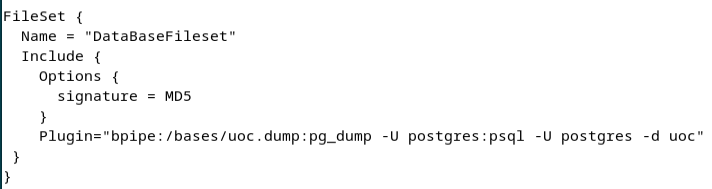
\includegraphics[width=0.5\linewidth]{instalacionBacula/filesetBpipe.png}
    \caption{Definición del FileSet para backups en Bacula.}
\end{figure}

Una vez definido el \textit{fileset}, procedemos a crear un nuevo trabajo de backup, especificando los detalles necesarios para su ejecución.

\textbf{Creación de un Trabajo de Backup}\medskip

Los detalles para la configuración del trabajo de backup son los siguientes:

\begin{itemize}
    \item \textbf{Nombre del trabajo:} DatabaseJOB
    \item \textbf{Habilitar trabajo:} Sí
    \item \textbf{Tipo por defecto:} Definición por defecto
    \item \textbf{Tipo de trabajo:} Backup
    \item \textbf{Nivel de backup:} Completo
    \item \textbf{Cliente a respaldar:} baculaCliente-fd
    \item \textbf{Conjunto de archivos a respaldar:} DataBaseFileset
    \item \textbf{Programación del backup:} Ciclo Semanal
    \item \textbf{Dispositivo de almacenamiento de destino:} StorageDaemon
    \item \textbf{Grupo de volúmenes:} Predeterminado
    \item \textbf{Destino de los mensajes:} Estándar
    \item \textbf{Prioridad del backup:} Predeterminada
\end{itemize}

\begin{figure}[H]
    \centering
    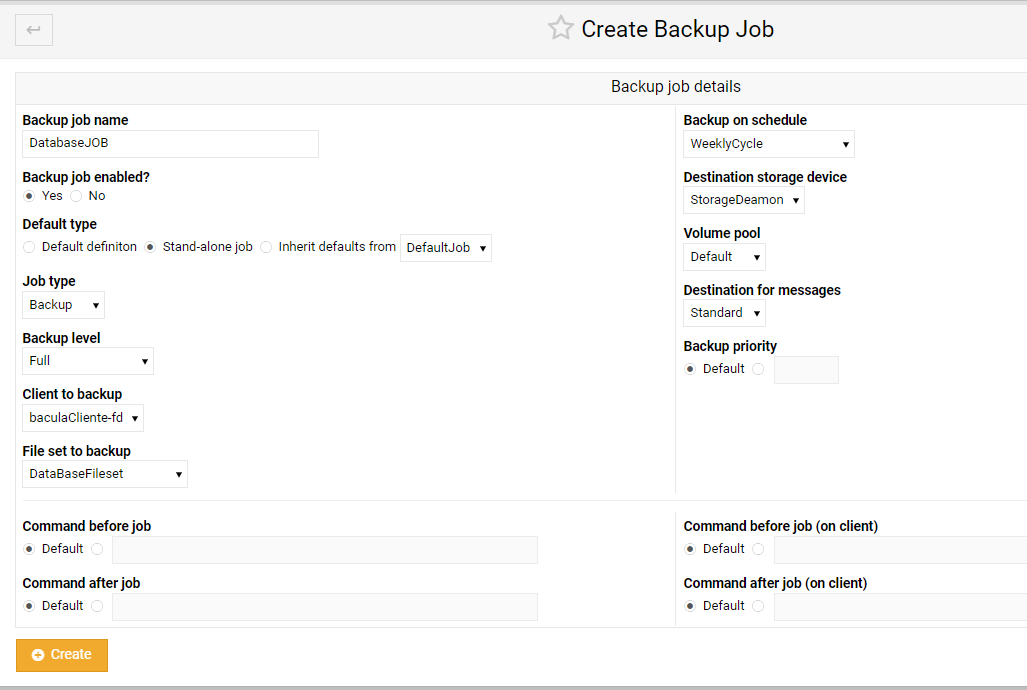
\includegraphics[width=0.5\linewidth]{instalacionBacula/databaseJOB.png}
    \caption{Detalles del trabajo de backup en Bacula.}
\end{figure}

\textbf{Eliminación de la Base de Datos}\medskip

A continuación, eliminamos la base de datos para simular una situación donde necesitemos restaurarla desde un backup:

\begin{figure}[H]
    \centering
    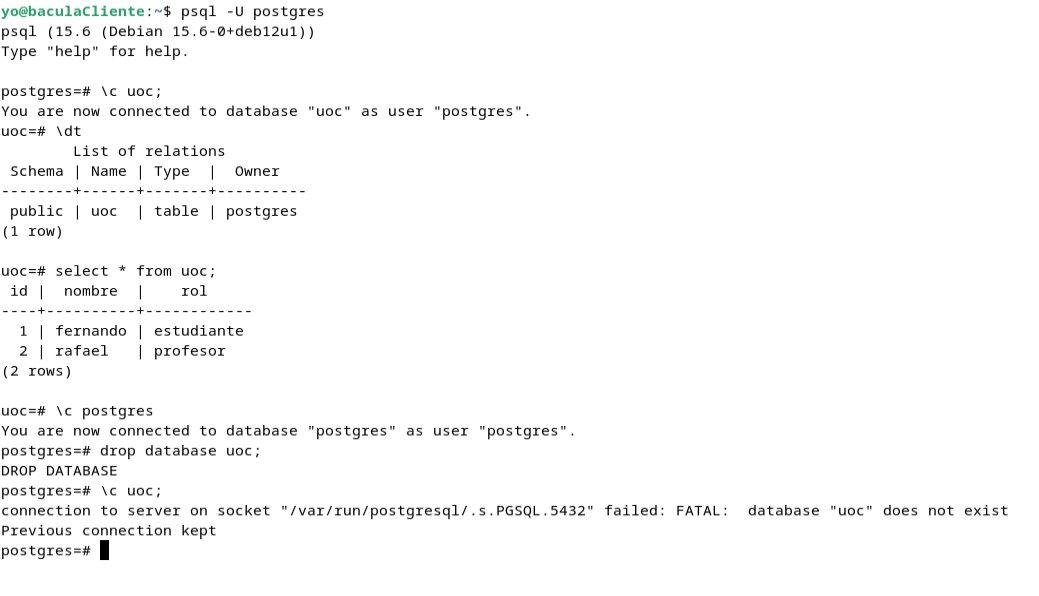
\includegraphics[width=0.5\linewidth]{instalacionBacula/dropdatabase.png}
    \caption{Comando para eliminar la base de datos \texttt{uoc}.}
\end{figure}

\textbf{Restauración de la Base de Datos}
\medskip

Realizamos la restauración de la base de datos y verificamos que las tablas sean restauradas correctamente:

\begin{figure}[H]
    \centering
    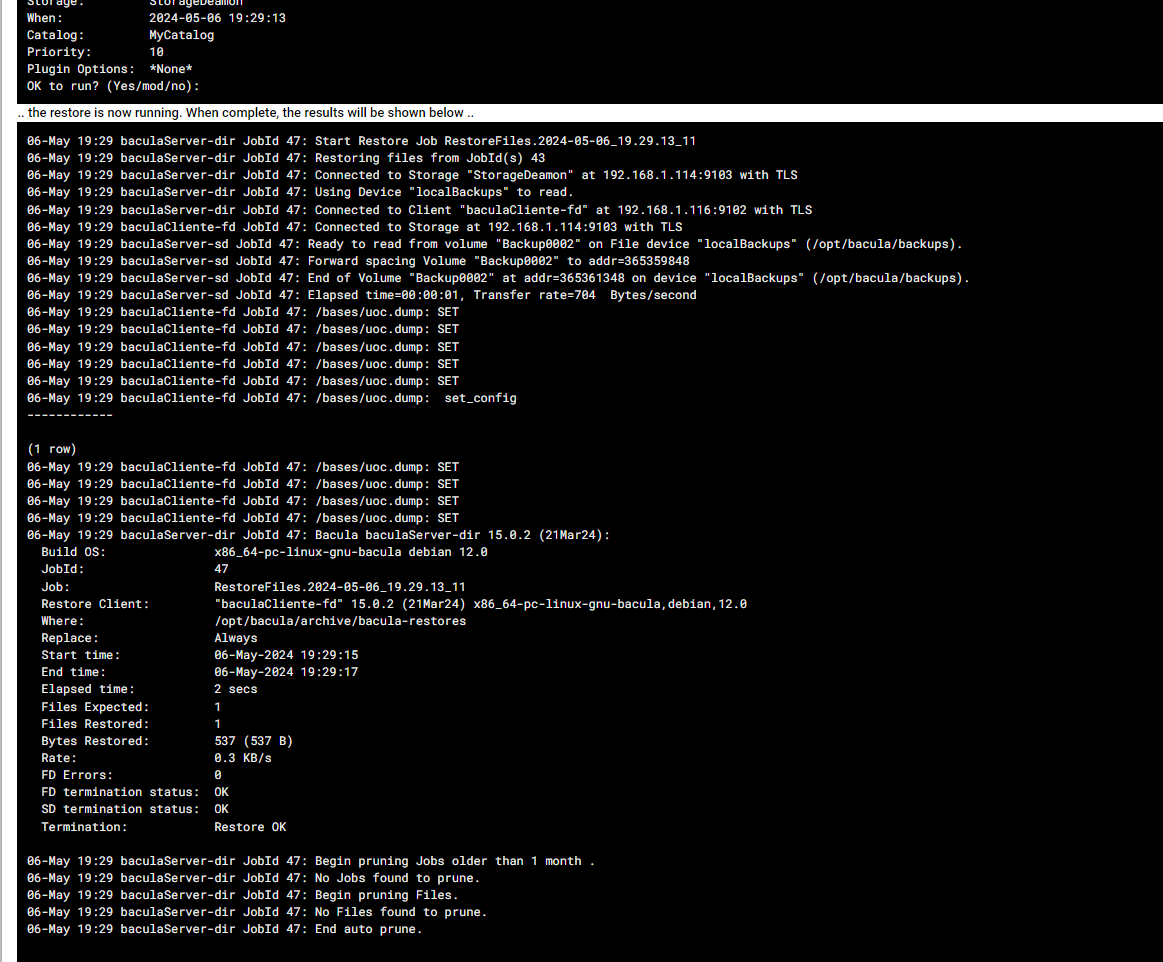
\includegraphics[width=0.5\linewidth]{instalacionBacula/restoreUOCdump.png}
    \caption{Proceso de restauración de la base de datos \texttt{uoc}.}
\end{figure}

Al finalizar la restauración, podemos confirmar que la tabla ha sido restaurada adecuadamente:

\begin{figure}[H]
    \centering
    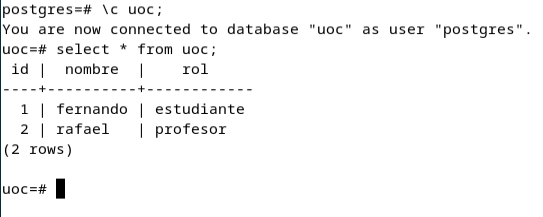
\includegraphics[width=0.5\linewidth]{instalacionBacula/restoreCompleteTABLAS.png}
    \caption{Tabla restaurada en la base de datos \texttt{uoc}.}
\end{figure}
